\documentclass[a4paper,12pt,fleqn]{article}
\usepackage[a4paper,mag=1000,includefoot,left=2cm,right=2cm,top=2.5cm,bottom=2cm]{geometry}
\usepackage[warn]{mathtext}
\usepackage[russian]{babel}
\usepackage{ucs}
\usepackage[utf8]{inputenc}
\usepackage{graphicx}
\usepackage{amsmath}
\usepackage{tabularx}
\usepackage{cite}
\usepackage{makecell}
\usepackage{booktabs}
\usepackage{pgfplotstable}
\usepackage{indentfirst} %Отступ в абзацах
\usepackage{doc}
% title
\author{Авдюшкин Василий}
\authortwo{Быковский Сергей}
\theme{Программа AUDIT}
\title{Руководство пользователя}
\begin{document}
% % Title here
\pagestyle{empty}
\maketitle
\newpage
\pagestyle{plain}
\tableofcontents
\newpage

\section{О программе}

Программа audit предоставляет графический интерфейс пользователя для взаимодействия с считывателем 
PR-G07 компании Parsec. Считыватель регистрирует происходящие события в специальной памяти,
называемой журналом транзакций. Программа считывает информацию из этого журнала и предоставляет её 
пользователю в виде таблицы в окне монитора, по которой можно осуществлять поиск необходимых данных. Результаты поиска,
при желании, возможно сохранить в файл отчета в формате csv, который без проблем открывается в Microsoft 
Office Excel.

Audit позволяет производить настройку устройства считывателя в окне настроек: задавать время реакции и дальность считывания
для 2 каналов, проводить синхронизацию внутренних часов, включать или отключать имеющиеся каналы.

Для удобства обработки полученной от считывателя информации, можно настроить реакцию на определенные 
события. Например, задать цвет, которым будет выделяться соответствующая запись в таблице монитора, или 
настроить оповещение оператора специальным сообщением, которое будет показываться при наступлении
определенных обстоятельств (обнаружение метки и т.п.). 

Все настройки, сделанные в программе, сохраняются в отдельном файле. Также сохраняется вся история 
событий, полученных от считывателя, и данные о реакциях оператора на сообщения. При закрытии программа
запоминает открытые файлы, а при открытии открывает их, тем самым восстанавливая рабочий сеанс пользователя.

\section{Главное окно}

Главное окно состоит всего из двух кнопок: <<Монитор>> и <<Настройки>> (рис. \ref{i:main}).
По нажатию на кнопку <<Настройки>>, открывается окно настроек, где возможно изменять настройки программы, 
а также настраивать подключенные к компьютеру считыватели. 

Окно монитора позволяет просматривать информацию
о новых событиях в табличном виде, а также проводить поиск по этой информации. В окне монитора
можно сохранить отфильтрованные данные о событиях в отчет, который затем можно открыть в Microsoft Office 
Excel и распечатать при необходимости.

\begin{figure}[h]
    \center{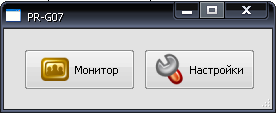
\includegraphics[scale=0.8]{img/main.png}}
    \caption{Главное окно}
    \label{i:main}
\end{figure}



\section{Окно настроек}

Окно настроек содержит элементы интерфейса, которые позволяют правильно настроить программу для
работы с устройством считывателя. Окно разделено на две части соответствующими вкладками: <<Файлы/Метки/События>> и
<<Подключенные устройства>>.

\subsection{Вкладка: Файлы/Метки/События}

Активировав вкладку
<<Файлы/Метки/События>>, пользователь получает возможность изменять настройки приложения. Верхние две строки вкладки
позволяют открыть или создать новые файлы журнала и настроек. 

\begin{center}
    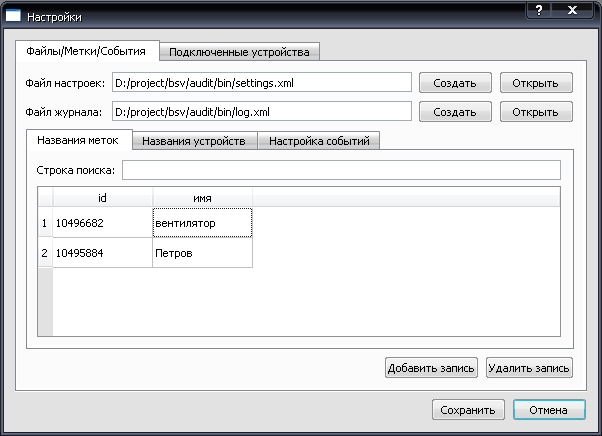
\includegraphics[scale=0.5]{img/settings_tag.png}
\end{center}

При открытии файла настроек, вся информация
из файла о настройках загружается в приложение и отображается в соответствующих местах интерфейса: информация о синонимах меток
ниже во вкладке <<Названия меток>>, информация о 
настройках реакций на события во вкладке <<Настройка событий>>. Программа также загружает данные о 
настройках устройств, ранее сконфигурированных в программе.

Для сохранения новых настроек приложения, необходимо нажать на кнопку <<Сохранить>> при активной вкладке
<<Файлы/Метки/События>>. При нажатии на кнопку <<Отмена>>, окно настроек закрывается.

При открытии файла журнала, информация о сохраненных в нем событиях отображается в окне монитора в виде таблицы.
Если файл хранит много данных, то показывается окно статуса процесса загрузки, где в процентах отображается
степень готовности операции чтения файла журнала.  

\subsubsection{Вкладка: Названия меток}

Для упрощения задач учета и контроля меток, в программе можно давать числовым идентификаторам меток
символьные имена. 

Вкладка <<Названия меток>> позволяет просматривать и редактировать информацию о синонимах меток. 
Редактирование осуществляется прямо в таблице, отображаемой во вкладке. Для удаления, необходимо выделить ненужную 
запись и нажать кнопку <<Удалить запись>>. Добавление новой записи производится посредством нажатия на
кнопку <<Добавить запись>>. Также в окне есть строка поиска, куда можно вводить ключевые слова, по которым
будет осуществлен поиск по таблице синонимов меток. Результаты поиска отобразятся сразу же в этой же таблице.

Чтобы сохранить изменения в файле настроек, нужно нажать кнопку <<Сохранить>>.

\subsubsection{Вкладка: Настройка событий}

Для выделения отдельных событий из всех случившихся, в программе можно настраивать определенную реакцию
на предполагаемое событие. 

Предусмотрено два вида событий: обнаружен новый таг либо таг потерян. На эти события возможно отреагировать двумя способами.
Либо выделить цветом событие в окне монитора, либо выдать сообщение о происшествии данного события.
В случае показа сообщения, программа регистрирует в файле журнала факт реакции оператора на него. Фиксируется закрытие
оператором окна с оповещением о событии.

Настройка реакций на события происходит путем редактирования таблицы в данной вкладке. Ячейки с именем устройства, именем метки, 
номером канала, событием и реакцией
изменяются посредством выпадающих списков. Причем при выборе реакции <<выделить цветом>>, открывается диалоговое окно с цветовой палитрой, где
пользователь может выбрать необходимый цвет подсветки события. 

В выпадающем списке выбора имени устройства отображаются только подключенные и обнаруженные программой устройства. Имя для метки можно выбрать из
выпадающего списка, который содержит синонимы, присвоенные меткам на вкладке "Файлы/Метки/События".
Ячейка с именем события изменяется как текстовое поле. 

Для удаления, необходимо выделить ненужную 
запись и нажать кнопку <<Удалить запись>>. Добавление новой записи производится посредством нажатия на
кнопку <<Добавить запись>>. 
Чтобы сохранить изменения в файле настроек, нужно нажать кнопку <<Сохранить>>.

\begin{center}
    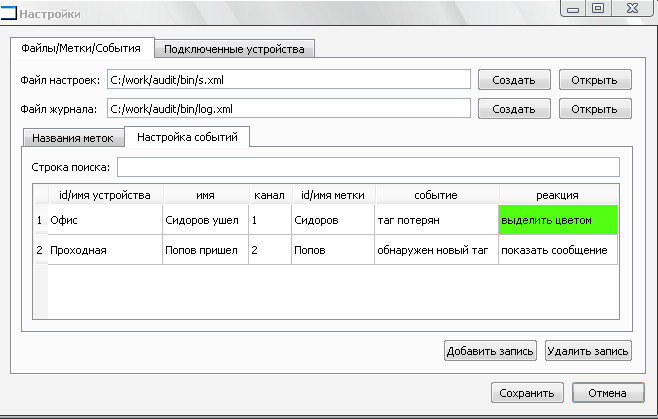
\includegraphics[scale=0.5]{img/settings_event.png}
\end{center}

\subsection{Вкладка: Подключенные устройства}

Элементы интерфейса на данной вкладке позволяют настраивать подключенные к компьютеру считыватели.
При нажатии на кнопку <<Найти устройства>>, программа отображает информацию о параллельно подключенных к USB портам устройствах в
виде списка в верхней части окна. 

\begin{center}
    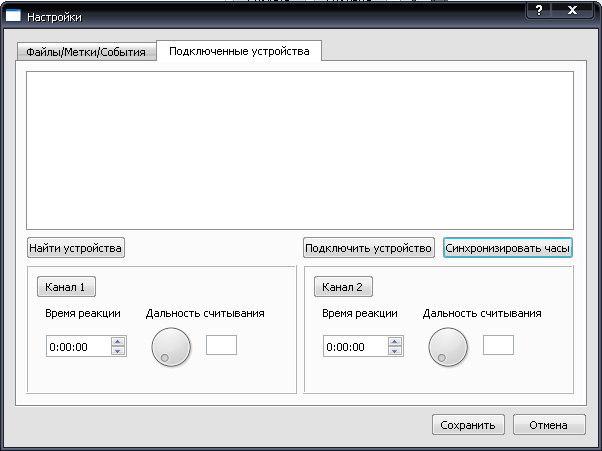
\includegraphics[scale=0.5]{img/settings_dev.png}
\end{center}

При нажатии на кнопку <<Синхронизировать часы>>, обновляется время внутренних часов для всех обнаруженных считывателей.
Чтобы поправить настройки для отдельного устройства, необходимо выбрать его щелчком левой клавиши мышки в списке.
После этого информация о текущих его настройках отобразится в нижней части окна. 
Подключение и отключение каналов происходит по нажатию на кнопках <<Канал 1>>, <<Канал 2>>.
Если канал включен, то соответствующая кнопка отображается в нажатом состоянии.

Для настройки расположенных последовательно на одной шине устройств необходимо добавить иформацию о них в таблицу. 
Для этого нужно дважды щелкнуть левой кнопкой мыши на строке с подключенным корневым устройством. Добавленному устройству
можно назначить адрес и имя. Имя устройства будет отображаться в таблице монитора при регистрации транзакций от данного считывателя.

Щелкнув правой кнопкой мыши на строке со считывателем, откроется контекстное меню дополнительных настроек. Это меню позваляет назначить новый
адрес устройству (при этом на шине должен находиться только один считыватель), получить (обновить) настройки или удалить устройство. 
Обновление настроек необходимо для загрузки в программу текущих настроек устройства 
(актуально когда подключается новый считыватель, настройки которого пока неизвестны программе).

\begin{center}
    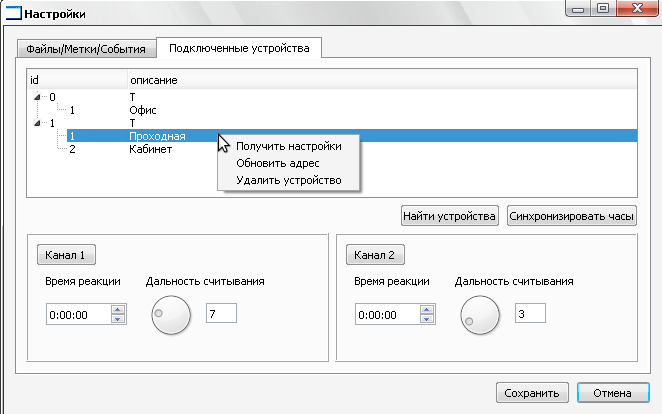
\includegraphics[scale=0.5]{img/settings_context.png}
\end{center}

После обнаружения устройств, программа начнет считывать данные из их журналов транзакций и 
отображать их в окне монитора. Подключение и отключение каналов происходит по нажатию на кнопках <<Канал 1>>, <<Канал 2>>.
Если канал включен, то соответствующая кнопка отображается в нажатом состоянии.

Настройка считывателя в соответствии с заданными параметрами производится после нажатия на кнопку <<Сохранить>>.
Если есть необходимость внести эти настройки в файл настроек, то нужно переключиться на вкладку <<Файлы/Метки/События>>
 и нажать на кнопку <<Сохранить>>.



\section{Окно монитора}

\subsection{Вкладка: Монитор}

Окно монитора отображает данные о произошедших событиях в табличном виде.
Чтобы просмотреть только информацию о метках, необходимо поставить флажок <<только информация о метках>>.
По нажатию на кнопку <<Очистить>>, происходит удаление всех записей в таблице монитора.
По нажатию на кнопку <<Сохранить>>, вызывается диалог с выбором имени файла для сохранения таблицы монитора в
csv файл, который легко открывается программой Microsoft Office Excel.

\begin{center}
    
\includegraphics[scale=0.5]{img/monitor.png}
\end{center}

\subsection{Вкладка: Параметры фильтрации}

На данной вкладке задаются параметры поиска событий в таблице монитора. 
При переключении на вкладку монитора, выполняется мгновенный поиск в соответствии с заданными параметрами.
Результаты отображаются в таблице монитора, которые можно сохранить в виде отчета в файл csv, а затем открыть и распечатать,
при необходимости, в Microsoft Office Excel.

\begin{center}
    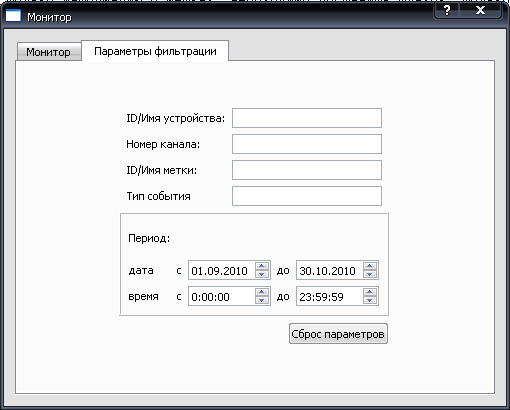
\includegraphics[scale=0.5]{img/monitor_find.png}
\end{center}

%\section{Возможные ошибки}

%%нет библиотек
%некорректный файл журнала
%ошибка обмена со считывателем

\end{document}